\documentclass[11pt,spanish,a4paper]{article}
% Versión 1.er cuat 2021 Víctor Bettachini < bettachini@df.uba.ar >

% Versión 1.er cuat 2021 Víctor Bettachini < bettachini@df.uba.ar >

\usepackage[T1]{fontenc}
\usepackage[utf8]{inputenc}

\usepackage[spanish, es-tabla]{babel}
\def\spanishoptions{argentina} % Was macht dass?
% \usepackage{babelbib}
% \selectbiblanguage{spanish}
% \addto\shorthandsspanish{\spanishdeactivate{~<>}}

\usepackage{graphicx}
\graphicspath{{./figuras/}}
% \usepackage{float}

\usepackage[arrowdel]{physics}
\newcommand{\pvec}[1]{\vec{#1}\mkern2mu\vphantom{#1}}
% \usepackage{units}
\usepackage[separate-uncertainty=true, multi-part-units=single, locale=FR]{siunitx}
\usepackage{isotope} % $\isotope[A][Z]{X}\to\isotope[A-4][Z-2]{Y}+\isotope[4][2]{\alpha}

\usepackage{tasks}
\usepackage[inline]{enumitem}
% \usepackage{enumerate}

\usepackage{hyperref}

% \usepackage{amsmath}
% \usepackage{amstext}
\usepackage{amssymb}

\usepackage{tikz}
\usepackage{tikz-dimline}
\usetikzlibrary{math}
\usetikzlibrary{arrows.meta}
% \usetikzlibrary{snakes}
% \usetikzlibrary{calc}
\usetikzlibrary{decorations.pathmorphing}
\usetikzlibrary{patterns}

\usepackage[hmargin=1cm,vmargin=1.6cm,nohead]{geometry}
% \voffset-3.5cm
% \hoffset-3cm
% \setlength{\textwidth}{17.5cm}
% \setlength{\textheight}{27cm}

\usepackage{lastpage}
\usepackage{fancyhdr}
\pagestyle{fancyplain}
\fancyhead{}
\fancyfoot{{\tiny \textcopyright DF, FCEyN, UBA}}
\fancyfoot[C]{ {\tiny Actualizado al \today} }
\fancyfoot[RO, LE]{Pág. \thepage/\pageref{LastPage}}
\renewcommand{\headrulewidth}{0pt}
\renewcommand{\footrulewidth}{0pt}


\begin{document}
\begin{center}
	\textbf{Física 2} (Físicos) \hfill \textcopyright {\tt DF, FCEyN, UBA}\\
	\textsc{\LARGE Difracción en un red de N rendijas}
\end{center}

Los ejercicios con (*) entrañan una dificultad adicional. Son para investigar después de resolver los demás.


\begin{enumerate}

\section*{Difracción por doble rendija}

\item 
\begin{enumerate}
	\item Se tienen dos rendijas iguales, de ancho $b$, cuya separación entre centros es $d$, colocadas entre dos lentes delgadas convergentes, ubicadas en forma simétrica respecto del eje óptico del sistema.
	Una fuente puntual monocromática que emite con $\lambda$ se encuentra en el foco de la primera lente. Considere la figura de interferencia--difracción de Fraunhofer de la fuente. 
	\begin{enumerate}
		\item Calcule la posición de los máximos y mínimos tanto de interferencia como de difracción. 
		\item Grafique la irradiancia sobre la pantalla, ¿en función de qué variable lo hace?
		¿Qué otra variable podría haber usado?
		\item Suponiendo que la teoría fuese exacta, ¿qué condiciones deberían cumplirse para que desaparezcan órdenes, y cuáles serían los órdenes desaparecidos? 
		\item ¿Cuántos órdenes de interferencia hay dentro de la campana principal de difracción?
		\item A la luz de estos resultados discuta el interferómetro de Young. 
		\item Considere que la fuente emite en $\lambda$, $2\lambda$ y $3\lambda$ simultáneamente.
		Para cada una de dichas longitudes de onda, ¿cuál es la posición de los máximos y mínimos de interferencia y difracción?
		En particular, ¿cuál es la posición del máximo principal?
	\end{enumerate}
	\item Repita lo hecho en (a), si la fuente se encuentra a una altura $h$ del eje óptico. 
	\item Idem (b) si el punto medio entre ranuras se encuentra a una altura $h'$ del eje óptico. 
\end{enumerate}


\item Se realiza una experiencia de difracción por doble rendija con una fuente que emite en \SI{4000}{\angstrom}.
La separación entre los puntos medios de las rendijas es de \SI{0.4}{\milli\metre} y el ancho de cada una de ellas es de \SI{0.04}{\milli\metre}.
La pantalla está a \SI{1}{\metre} de las rendijas.
Luego se cambia la fuente por otra que emite en \SI{6000}{\angstrom}.
Determine:
\begin{enumerate}
	\item En cuánto varió la interfranja. 
	\item En cuánto varió el número total de franjas de interferencia contenidas en la campana principal de difracción. 
	\item En cuánto varió el ancho angular de la campana principal de difracción. 
\end{enumerate}



\item Sobre dos ranuras separadas una distancia de \SI{1}{\milli\metre} incide la superposición de dos ondas planas monocromáticas de longitudes de onda $\lambda_1$ y $\lambda_2$
\begin{enumerate}
	\item ¿Qué relación debe satisfacer el cociente $\lambda_1/\lambda_2$ para que el tercer orden de interferencia constructiva de $\lambda_1$ coincida con el tercer mínimo de $\lambda_2$? 
	\item ¿Qué ancho deben tener las ranuras para que además esos órdenes coincidan con el primer mínimo de difracción de $\lambda_1$?
	¿Qué irradiancia se registrará en la pantalla en ese punto? 
\end{enumerate}

\section*{Redes de N rendijas}

\item Una onda plana monocromática de longitud de onda $\lambda$ incide normalmente sobre una red de transmisión plana formada por $N$ rendijas de ancho $b$ y período $d$.
Suponiendo que la teoría corresponde a una descripción exacta del fenómeno: 
\begin{enumerate}
	\item Analice la distribución de irradiancia sobre la pantalla y grafíquela.
	\item Calcule:
	\begin{enumerate}
		\item La posición angular de las líneas espectrales (¿a qué máximos corresponden?), y su irradiancia.
		\item El número de mínimos de interferencia entre dos líneas espectrales, por ende, ¿cuántos máximos secundarios hay?
		\item El ancho angular de las líneas espectrales.
		\item El máximo orden observable. 
	\end{enumerate}
	\item Discuta: 
	\begin{enumerate}
		\item ¿Qué aproximación hace en los ángulos?
		\item La dependencia de los parámetros con el número de rendijas y con la densidad de rendijas. 
	\end{enumerate}
\end{enumerate}



\item Sobre la red del problema anterior incide la superposición de dos ondas planas monocromáticas de longitudes de onda $\lambda$ y $\lambda+\Delta\lambda$.
\begin{enumerate}
	\item Calcule la dispersión angular, el poder resolvente, y el máximo del mismo.
	\item Grafique la irradiancia sobre la pantalla. 
	\item Recalcule el problema anterior para una incidencia distinta de la normal, y discuta si existe alguna ventaja al trabajar de esa manera. 
\end{enumerate}



\item 
\begin{minipage}[t][3.3cm]{0.6\textwidth}
Se tiene un dispositivo como el que se muestra en la figura, formado por una red dispuesta entre dos lentes. La red es iluminada por dos fuentes $S_1$ y $S_2$ que emiten luz con la misma irradiancia, pero con longitudes de onda $\lambda_1$ y $\lambda_2$ respectivamente.
Se sabe que la red es de rendijas, pero no se conocen su número \(N\), ancho \(b\) o período de la red \(d\).
\end{minipage}
\begin{minipage}[c][0cm][t]{0.35\textwidth}
	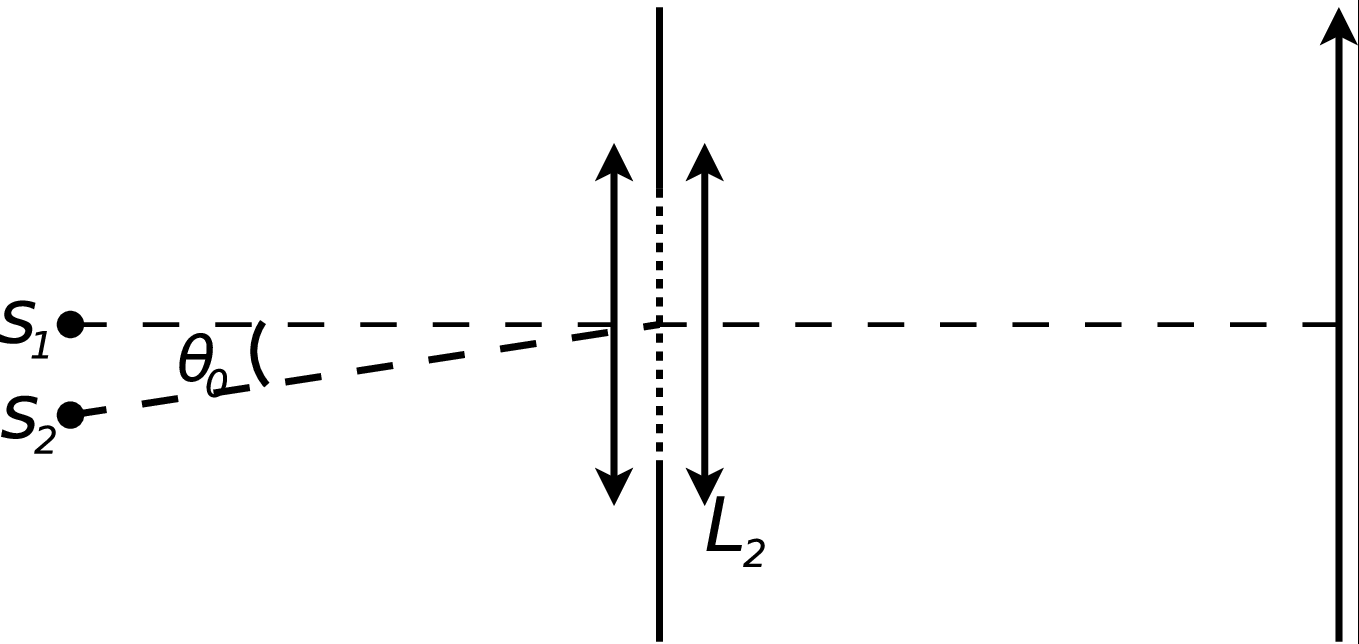
\includegraphics[width=\textwidth]{ej5-43}
\end{minipage}
Para poder caracterizarla, se realizan observaciones de la figura de difracción--interferencia producida en el plano de observación.
A partir de lo cual se logra determinar que:
\begin{itemize}
	\item El orden \num{-1} de interferencia correspondiente a $\lambda_2$ se encuentra una distancia $a_0= \SI{0.1}{\milli\metre}$ por encima del orden \num{+1} correspondiente a $\lambda_1$. 
	\item El ancho de la campana de difracción correspondiente a $\lambda_1$ es $d_0= \SI{10}{\centi\metre}$.
\end{itemize}
Realizar lo siguiente con los datos: distancia focal de la lente $L_2 = \SI{3}{\metre}$; $\lambda_1 = \SI{4000}{\angstrom}$ y $\lambda_2 = \SI{5000}{\angstrom}$.
\begin{enumerate}
	\item Dar la expresión para la distribución de irradiancia que se observa en la pantalla y justificar por qué la escribe así.
	Hacer un gráfico muy cualitativo de dicha distribución (que dé una idea básica de lo que se va a observar).
	\item Determinar las posiciones angulares de todos los ceros de interferencia y difracción. 
	\item Determinar las posiciones de los órdenes de interferencia.
	\item Encontrar los parámetros de la red $b$ y $d$. 
	\item Ambos órdenes (¡cuidado; se trata de órdenes diferentes!) están suficientemente separados entre sí, según el criterio de Rayleigh.
	Hallar una cota	para $N$. 
\end{enumerate}


\end{enumerate}

\end{document}
